\documentclass[main.tex]{subfiles}


\begin{document}


\subsection{Frameshift stimulating elements of multiple coronaviruses form long-range RNA--RNA interactions}

Within the genomes of many RNA viruses, long-range RNA--RNA interactions regulate core processes such as viral protein synthesis~\cite{Nicholson2014}.
In SARS coronavirus 2 (SARS-CoV-2), the frameshift stimulating element (FSE) base pairs with another genomic element over 1,000 nt downstream~\cite{Ziv2020}.
For its length, this RNA--RNA interaction appears surprisingly favorable, forming in approximately half of the genomic RNA molecules within infected cells~\cite{Lan2022}.
Although the FSE is essential for synthesizing five viral proteins including the RNA polymerase, the function (if any) of the long-range interaction it forms remains unknown~\cite{Allan2023}.

We hypothesized that if the long-range interaction is functional, then other SARS-related viruses -- and potentially more distantly related coronaviruses -- would feature similar long-range interactions involving their FSEs.
To test this hypothesis, we performed SEARCH-MaP with FSE-targeted ASOs on 1,799 nt segments from eight selected coronaviruses.


\subsubsection{Computational and experimental screening identifies eight coronaviruses with potential long-range interactions}

As of December 2021, the NCBI Reference Sequence Database~\cite{OLeary2016} contained sixty-two complete genomes of coronaviruses.
To focus on those likely to have long-range interactions involving the FSE, we predicted the likelihood that each base in a 2,000 nt section surrounding the FSE would pair with a base in the FSE.
Based on these predicted interactions (SFIG), we selected ten coronaviruses (including SARS-CoV-2) for further study -- at least one from each genus.
Within the genus \textit{Betacoronavirus}, we included all three of the SARS-related viruses -- SARS coronaviruses 1 (\verb|NC_004718.3|) and 2 (\verb|NC_045512.2|) and bat coronavirus BM48-31 (\verb|NC_014470.1|) -- because they clustered into their own structural outgroup, distinct from all other coronaviruses.
The other three strains of \textit{Betacoronavirus} that we selected were MERS coronavirus (\verb|NC_019843.3|) with a predicted interaction at positions 510-530; and human coronavirus OC43 (\verb|NC_006213.1|) and murine hepatitis virus strain A59 (\verb|NC_048217.1|), both with a predicted upstream interaction at positions 10-20.
We selected two strains of \textit{Alphacoronavirus}: transmissible gastroenteritis virus (\verb|NC_038861.1|) and bat coronavirus 1A (\verb|NC_010437.1|), predicted to have interactions at positions 440-460 and 350-360, respectively.
Avian infectious bronchitis virus strain Beaudette (\verb|NC_001451.1|) -- a strain of \textit{Gammacoronavirus} -- was predicted to have a strong interaction at positions 330-350, while common moorhen coronavirus HKU21 (\verb|NC_016996.1|) was the species of \textit{Deltacoronavirus} with the most promising FSE interactions.

We reasoned that if an FSE does interact with a distant RNA element, then removing that element by truncating the RNA would break the interaction, causing a structural change in the FSE that could be detected though chemical probing.
For each of the ten coronaviruses that passed the computational screen, we \textit{in vitro} transcribed and performed DMS-MaPseq~\cite{Zubradt2016} on both a 239 nt ("short") segment comprising the FSE and minimal flanking sequences and a 1,799 nt ("long") segment encompassing the FSE and all sites with which it was predicted to interact.
All coronaviruses except for human coronavirus OC43 and MERS coronavirus showed differences in their DMS reactivity profiles between the short and long segments (SFIG), suggesting long-range interactions between the FSE and another element within the long segment.


\subsubsection{SEARCH-MaP reveals long-range interactions involving the FSE in four coronaviruses}

To determine whether the FSE forms a long-range interaction with another RNA element -- and if so, which element -- in each coronavirus, we performed SEARCH-MaP on the 1,799 nt RNA segment using FSE-targeted ASOs.
We computed the Spearman correlation using a sliding window between the DMS reactivities with and without ASOs (Figure \ref{fig3}).
[HOW MANY] coronaviruses 

\begin{figure}[H]
	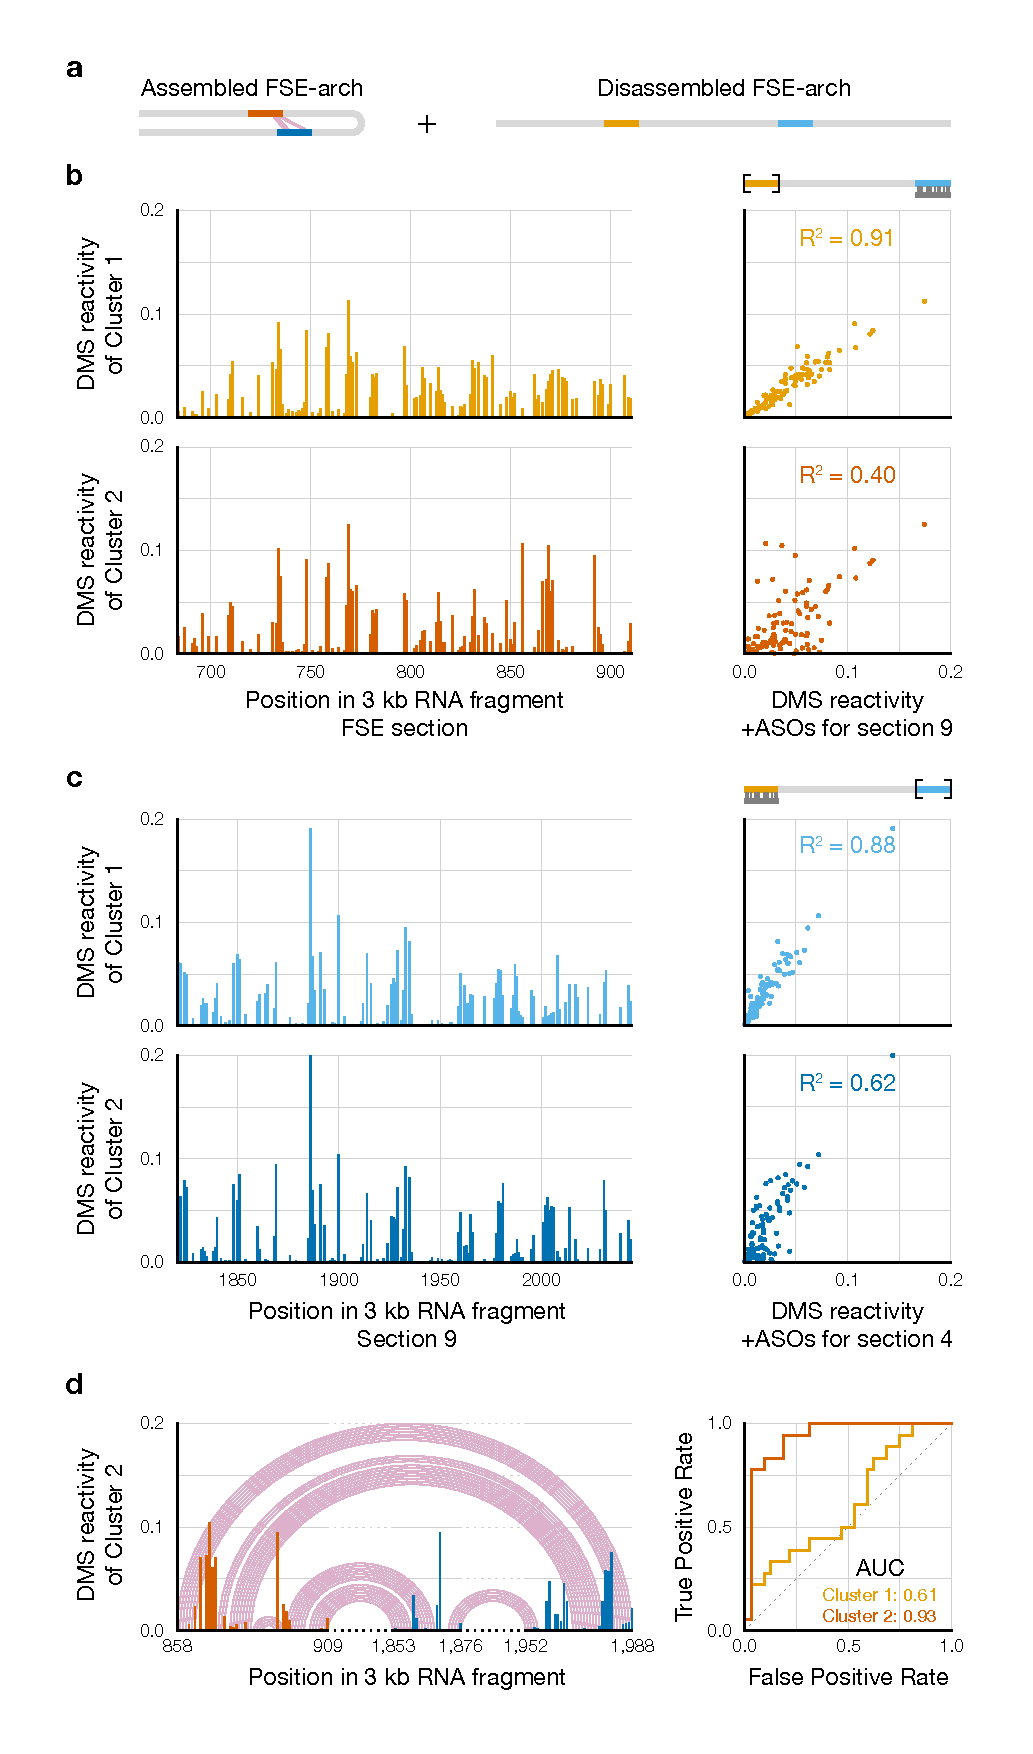
\includegraphics[height=0.95\textheight]{../MainFigures/fig3.pdf}
	\caption{}
	\label{fig3}
\end{figure}


\end{document}
